%  !TEX root = ../main.tex

\begin{figure}
    \centering
    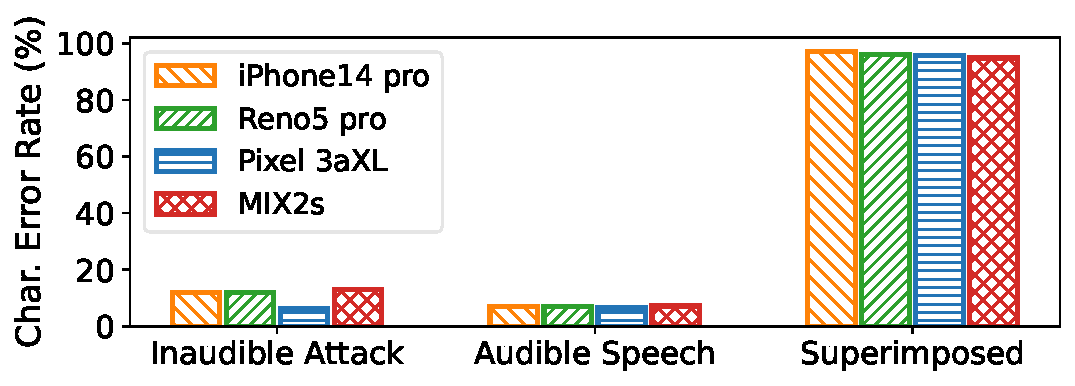
\includegraphics[width=0.45\textwidth]{preliminary_cer.pdf}
    \caption{CER of four recording devices under three settings. }
    \label{fig:preliminary_wer}
    \vspace{-10pt}
\end{figure}

\section{Preliminary Investigation}\label{sec:preliminary}
\subsection{\blue{Failure of Traditional Inaudible Attacks}}\label{pre_inaudible_attack}
\blue{
Given the purpose of avoiding alerting users, directly injecting malicious commands into ASR systems using laser-~\cite{sugawara2020light} or ultrasound-based~\cite{zhang2017dolphinattack,roy2018inaudible} inaudible attacks is intuitive. Although laser-based attacks can reach an 100m attack range, we choose ultrasound instead of laser for three practical reasons: (1) The laser spot on the microphone is visible and will alert users immediately; (2) The laser-based attack requires strict line-of-sight alignment; and (3) The severe channel distortion of laser-delivered attacks may nullify fine-grained adversarial perturbations.}

\blue{
To examine whether traditional ultrasound-based attacks can manipulate ASRs into recognizing the modulated malicious commands while users are speaking, we need to ensure that the ultrasonic carrier frequency is optimal. Therefore, we first employ an ultrasonic Vifa~\cite{vifa} to launch a wide-range carrier sweeping from 20$\sim$40~kHz. By analyzing the signal-to-noise ratio (SNR) of demodulated basebands, we justify the optimal frequency of four recording devices, i.e., iPhone14 pro: 24.7~kHz, Reno5 pro: 27.7~kHz, Pixel 3aXL: 25.6~kHz, and MIX2s: 25.1~kHz, respectively. This result is consistent with DolphinAttack~\cite{zhang2017dolphinattack}, which reveals most devices' optimal attack carrier frequency is around 25~kHz (22.6$\sim$27.9~kHz). In this way, we set the default carrier frequency to 25~kHz, whose advantages are two-fold: (1) Due to lower airborne attenuation, 25~kHz also benefits longer-range attacks than high-frequency carriers (e.g., 40kHz); (2) Moreover, 25~kHz as one of the most typical parameters for commercial ultrasonic transducers that cost as low as 0.14\$ per unit~\cite{25kHz_ultra_transducer}, making the attack cost-effective.
}

\blue{
Although the optimal attack frequency is determined, traditional ultrasound-based attacks still fail due to \textit{user disruption}. Specifically, we select 10 text-to-speech commands listed in Tab.~\ref{tab:diff_commands} (e.g., ``turn on airplane mode'') as the basebands. 
Four smartphones 50~cm away serve as recording devices that recover the AM signal into audible-band speech. 
For benign command samples, we randomly select 20 utterances from the popular fluent speech commands dataset~\cite{fluent2020commands} to be played via a loudspeaker and recorded by identical smartphones.
We also perform simultaneous emissions of both signals, so they are superimposed on each other. 
For each recording device, we collected $10\times20=200$ mixed samples and calculated each sample's character error rate (CER) through the Azure speech-to-text API~\cite{azureasr}. As shown in Fig.~\ref{fig:preliminary_wer}, the direct ultrasound-based attacks and benign audio are well recognized by ASR models, with average CER of 10.8\% and 6.88\%, respectively. Nevertheless, once attack emission and user's voice coincide, the attack performance (i.e., 10 malicious commands as the target transcription) will severely degrade to an average CER up to 96.01\%, even if we have boosted its power\footnote{To facilitate ultrasound-based attacks, we set the volume up to 95 dB, and that of audible benign speech is 70$\sim$75 dB.}. We believe it is a consequence that when ASRs process the mixed samples, each sampling point of the malicious signal sequence is affected by the human voice, making the acoustic features extracted by the ASR deviate from adversaries' anticipation.}

